\section{Protocolo de transmisión}
	\subsection{Descripción del problema}
	Desarrollar un programa que genere 50 cadenas de 32 caracteres que sean guardadas en un archivo, para después ser evaluadas por un autómata, en este caso el autómata de paridad binaria y guardar las cadenas binarias en otro archivo, siguiendo el siguiente diagrama.
	\begin{figure}[ht]
		\begin{center}
			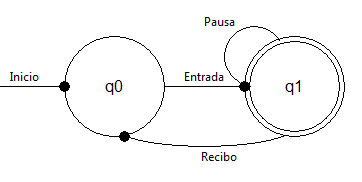
\includegraphics[width=10cm, height=5cm]{img/protocolo.png}
			\caption{Diagrama de transiciones del autómata. \cite{WEB}}
			\label{fig:diagrama3}
		\end{center}
	\end{figure}
	\subsection{Código}
	El código fue realizado en Python 3.5.
	\subsection{Pruebas}
	Pruebas de las opciones del menú.
	{\large Modo automático.}
	{\large Diagrama.}